\documentclass[a4paper,11pt]{article}

% Use utf-8 encoding for foreign characters
\usepackage[utf8]{inputenc}
\usepackage[british,english]{babel}
\usepackage[T1]{fontenc}

% Setup for fullpage use
\usepackage{fullpage}

% Multipart figures
\usepackage{subfigure}

% More symbols
\usepackage{amsmath}
\usepackage{amssymb}
\usepackage{latexsym}

% For pretty URLs, see: http://en.wikibooks.org/wiki/LaTeX/Hyperlinks
\usepackage{hyperref}

% Surround parts of graphics with box
\usepackage{boxedminipage}

% Package for including code in the document
\usepackage{listings}

% If you want to generate a toc for each chapter (use with book)
\usepackage{minitoc}

% Uncomment if you want to use Palatino as font
\usepackage[sc]{mathpazo}
\linespread{1.05}         % Palatino needs more leading (space between lines)

% This is now the recommended way for checking for PDFLaTeX:
\usepackage{ifpdf}


\addto\captionsenglish{\renewcommand{\refname}{}}

%\newif\ifpdf
%\ifx\pdfoutput\undefined
%\pdffalse % we are not running PDFLaTeX
%\else
%\pdfoutput=1 % we are running PDFLaTeX
%\pdftrue
%\fi

\ifpdf
\usepackage[pdftex]{graphicx}
\else
\usepackage{graphicx}
\fi
\title{Deliverable 6: Sprint \#4\\\small{for}\\\small{Danske Bank: Peer-to-peer}}
\author{ Group Delta:\\Jesper Borgstrup, Thomas Kjeldsen and Mads Ohm Larsen }

\date{May 20, 2011}

\begin{document}

\ifpdf
\DeclareGraphicsExtensions{.pdf, .jpg, .tif}
\else
\DeclareGraphicsExtensions{.eps, .jpg}
\fi

\maketitle

%\tableofcontents
%\vspace{2cm}

%%%%%%%%%%%%%%%%%%%%%%%%%%%%%%%%%%%%%%
%%%%%%%%%%%%%%%%%%%%%%%%%%%%%%%%%%%%%%
%%%%%%%%%%%%%%%%%%%%%%%%%%%%%%%%%%%%%%

\section{Requirements for this deliverable}
\begin{enumerate}
\item Doing a demo in class (on 2011-05-18)
\item Giving us access to your source code
\item Handing in a collection of your sprint material
\item Describing a sprint retrospective (e.g., as a set of bullets outlining what
when well, what went wrong, and how you will improve for the next sprint)
\end{enumerate}

The Sprint Demo was given on May 18th. This document describes requirements 2-4 as well as the sprint learning goal -- mutual code inspection in our group and group Bravo.

%%%%%%%%%%%%%%%%%%%%%%%%%%%%%%%%%%%%%%
%%%%%%%%%%%%%%%%%%%%%%%%%%%%%%%%%%%%%%
%%%%%%%%%%%%%%%%%%%%%%%%%%%%%%%%%%%%%%

\section{Inspection}
%%%%%%%%%%%%%%%%%%%%%%%%%%%%%%%%%%%%%%
%%%%%%%%%%%%%%%%%%%%%%%%%%%%%%%%%%%%%%
%%%%%%%%%%%%%%%%%%%%%%%%%%%%%%%%%%%%%%

\section{Source code access}
Our source code is publicly available on GitHub from \url{https://github.com/omegahm/DBP2P}.

If you wish to checkout our code (read-only) using Git, then use git clone with this URL:
\url{git://github.com/omegahm/DBP2P.git}

%%%%%%%%%%%%%%%%%%%%%%%%%%%%%%%%%%%%%%
%%%%%%%%%%%%%%%%%%%%%%%%%%%%%%%%%%%%%%
%%%%%%%%%%%%%%%%%%%%%%%%%%%%%%%%%%%%%%

\section{Sprint material}
Sprint Material needed to assess our progress include the following:
\begin{itemize}
\item source code (version number and access method is sufficient)
\item product backlog (before and after the sprint)
\item sprint backlog
\item any other material (e.g., burndown chart) that illustrates your progress
\end{itemize}


\subsection{Source Code}

%The final product of sprint \#4 has been tagged \href{https://github.com/omegahm/DBP2P/tree/sprintdemo2}{\tt sprintdemo3}. in the git repository, where the application is located in the folder {\tt DustyTubaSampleApp}.

%The following main tasks have been completed during this sprint:
%\begin{itemize}
%	\item ``Libraryfying'' our code
%	\item Using the library to establish Bluetooth connection (2.1+ devices only)
%	\item Wrote documentation
%	\begin{enumerate}
%		\item Both for future developers of the library, as well as for users of the library
%	\end{enumerate}
%\end{itemize}

%In regards to our user stories, the tasks completed correspond to the following user stories:
%\begin{verbatim}
%  As a        customer of the API
%  I want to   be able to decide the data structure of the information
%  Such that   I can structure the messages according to my needs
%\end{verbatim}
%
%\subsection{Product Backlog}
%Our sprint backlog is shown in figure \ref{productbacklog} on page \pageref{productbacklog}.
%
%% \begin{figure}[ht!]
%% 	\begin{center}
%% 	% Insert sprint backlog here
%% 	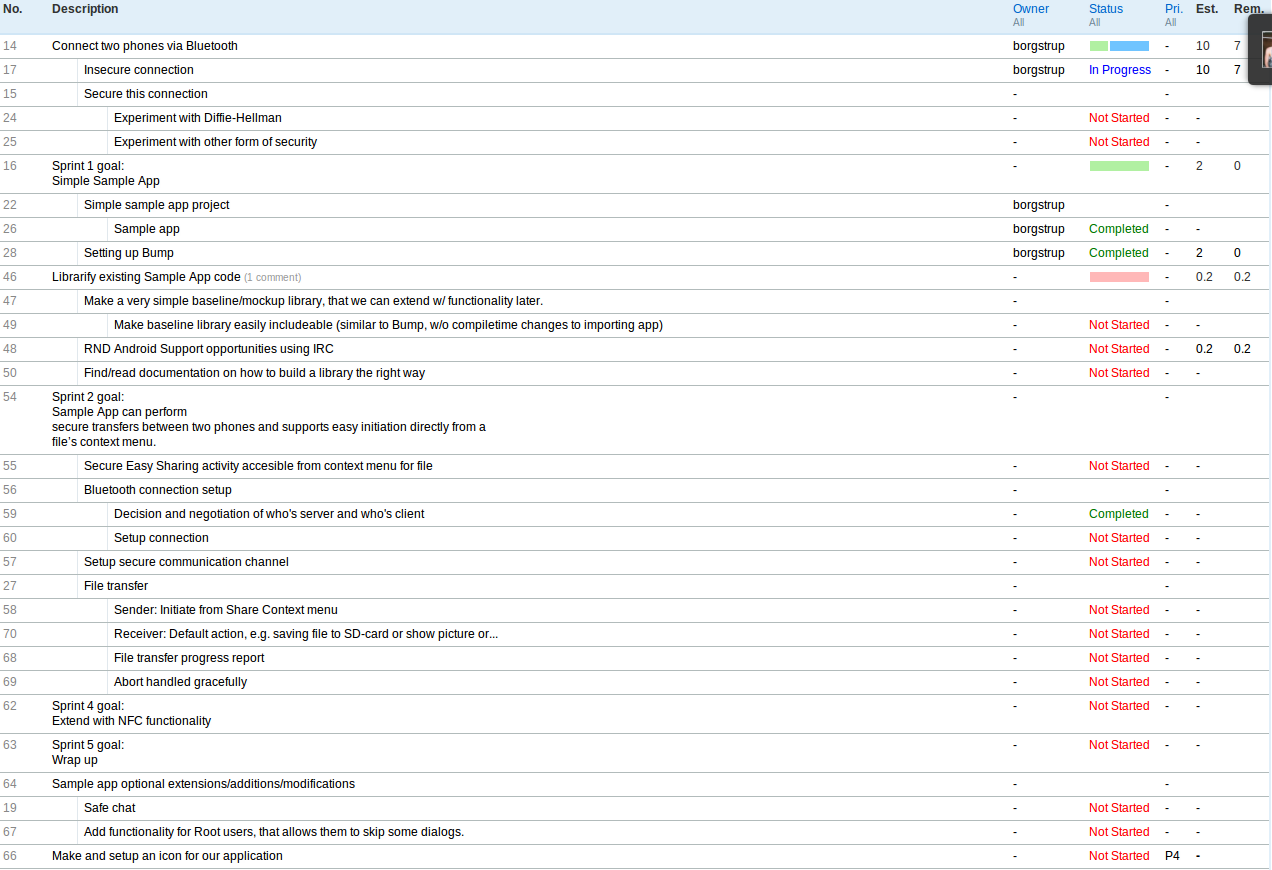
\includegraphics[width=0.9\textwidth]{productbacklog.png}		
%% 	\end{center}
%% 	\caption{Our product backlog at the end of sprint \#2.}
%% 	\label{productbacklog}
%% \end{figure}
%
%\subsection{Sprint Backlog}
%Our sprint backlog is shown in figure \ref{sprintbacklog} on page \pageref{sprintbacklog}.
%
%% \begin{figure}[ht!]
%% 	\begin{center}
%% 	% Insert sprint backlog here
%% 	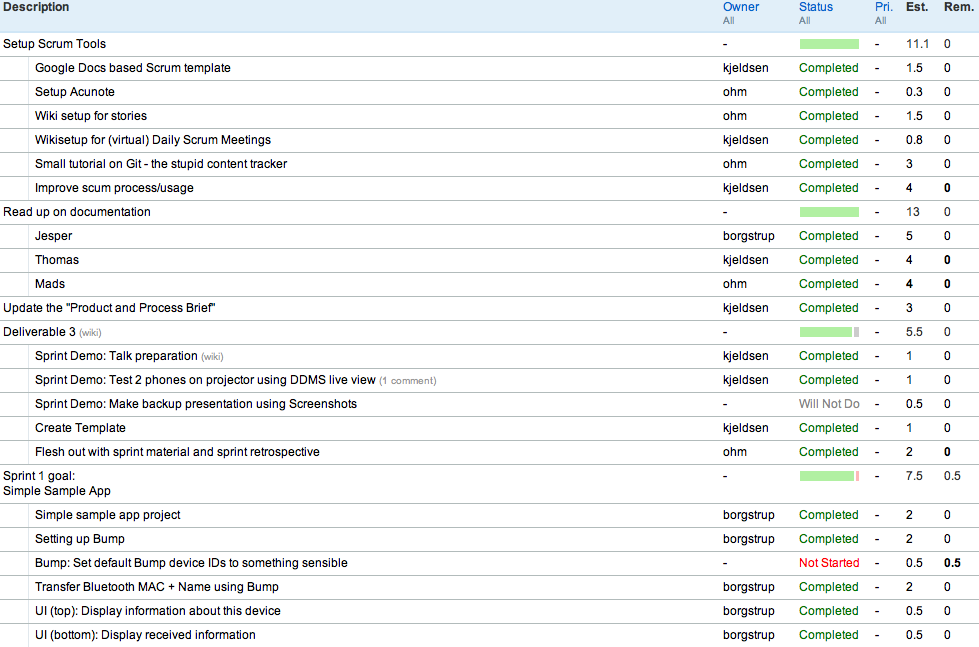
\includegraphics[width=0.85\textwidth]{sprintbacklog.png}		
%% 	\end{center}
%% 	\caption{Our sprint backlog after the sprint was finished}
%% 	\label{sprintbacklog}
%% \end{figure}
%
%\subsection{Burndown chart}
%
%Our burndown chart is shown in figure \ref{burndown} on page \pageref{burndown}.
%
%% \begin{figure}[ht!]
%% 	\begin{center}
%% 	% Insert burndown chart here
%% 	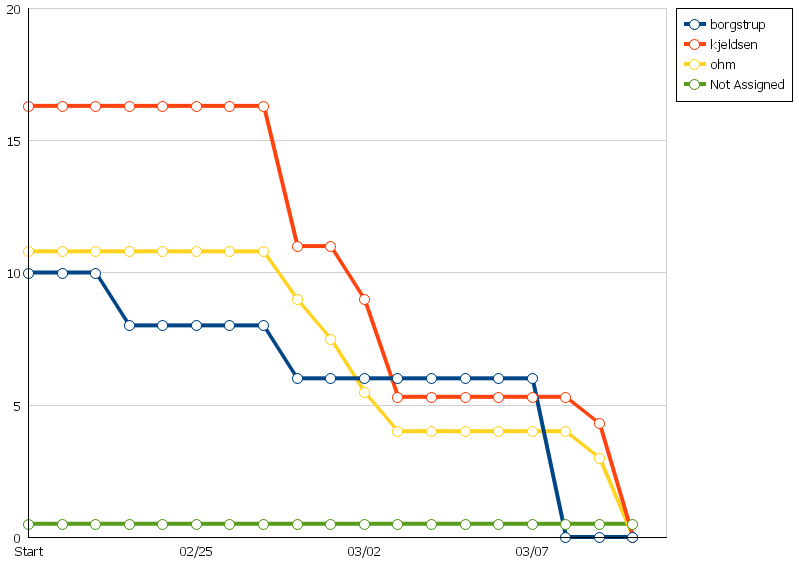
\includegraphics[width=\textwidth]{burndown.png}		
%% 	\end{center}
%% 	\caption{Our burndown chart at the end of the sprint}
%% 	\label{burndown}
%% \end{figure}
%
%\subsection{Acunote}
%We have got an Acunote account\footnote{\url{http://dbp2p.acunote.com/}} setup, and %access to this have been granted.
%
%\clearpage
%
%%%%%%%%%%%%%%%%%%%%%%%%%%%%%%%%%%%%%%
%%%%%%%%%%%%%%%%%%%%%%%%%%%%%%%%%%%%%%
%%%%%%%%%%%%%%%%%%%%%%%%%%%%%%%%%%%%%%

\section{Sprint retrospective}



\end{document}
